\section{kubernetes基本组成}
kubernetes主要分为2种角色:master和node。其中,master包含了kube-apiserver,kube-scheduler和
kube-controller-manager;而node则包含了kubelet和kube-proxy。当然,可以把master和node节点混合
在一起。每个服务的角色和用途不一样。
\begin{itemize}
    \item kube-apiserver:提供api访问请求控制,访问etcd和转发etcd的访问控制请求。用户自己做Active-Active模式。
    \item kube-scheduler:负责pod的调度。默认Active-Backend模式
    \item kube-controller-manager:包含Node,route,service和volume等控制器。默认Active-Backend模式
    \item kubelet:控制pod(容器)。只负责当前节点,单点。
    \item kube-proxy:负责为Service提供cluster内部的服务发现和负载均衡。只负责当前节点,单点。
\end{itemize}

创建一组pod时,其内部大致流程如图 \nameref{fig:create_pod}所示
\begin{figure}[H]
  \centering
  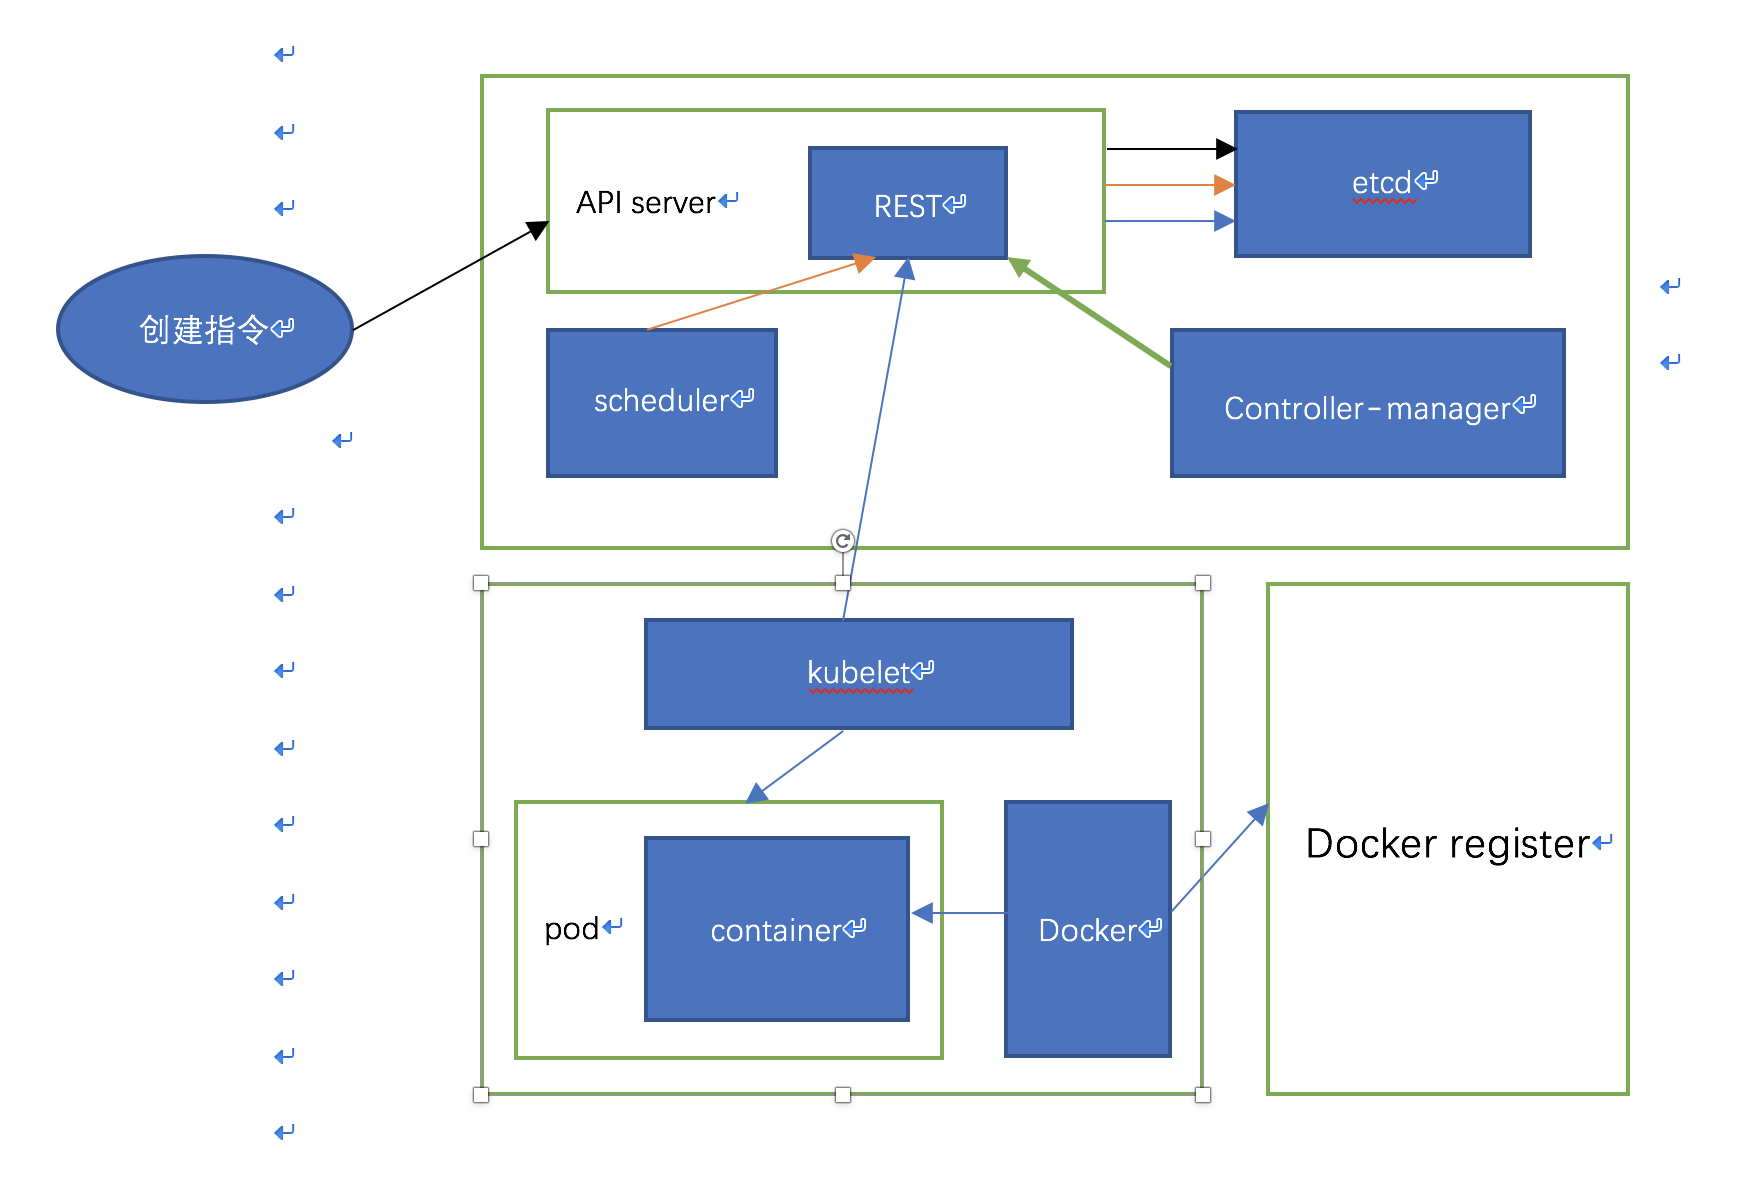
\includegraphics[scale=0.5]{create_pod.png}
  \caption{新建pod}
  \label{fig:create_pod}
\end{figure}

\begin{enumerate}
    \item 指令传到APIserver,API server将pod的创建信息固化到etcd上
    \item scheduler监控APIserver的watch端口,查看到etcd中有创建pod的消息,下面就为pod选择合适的node节点,并进行绑定,绑定成功后,scheduler会调用APIServer的API的增加接口在etcd中创建一个boundpod对象,描述在一个工作节点上绑定运行的所有pod信息
    \item kubelet监控APIserver的watch端口监听pod信息,发现有新的pod绑定在该节点上的时候,则根据etcd中的boundpod信息进行pod创建
    \item docker会从image仓库中查看docker的信息,并下载docker image最终进行container的创建
    \item controller-manager会监听API server的端口,对node、pod副本、资源等进行管理
\end{enumerate}

而通过外部访问pod时,其内部流程又存在一些区别,其大致如图\nameref{fig:visit_pod}所示
\begin{figure}[H]
    \centering
    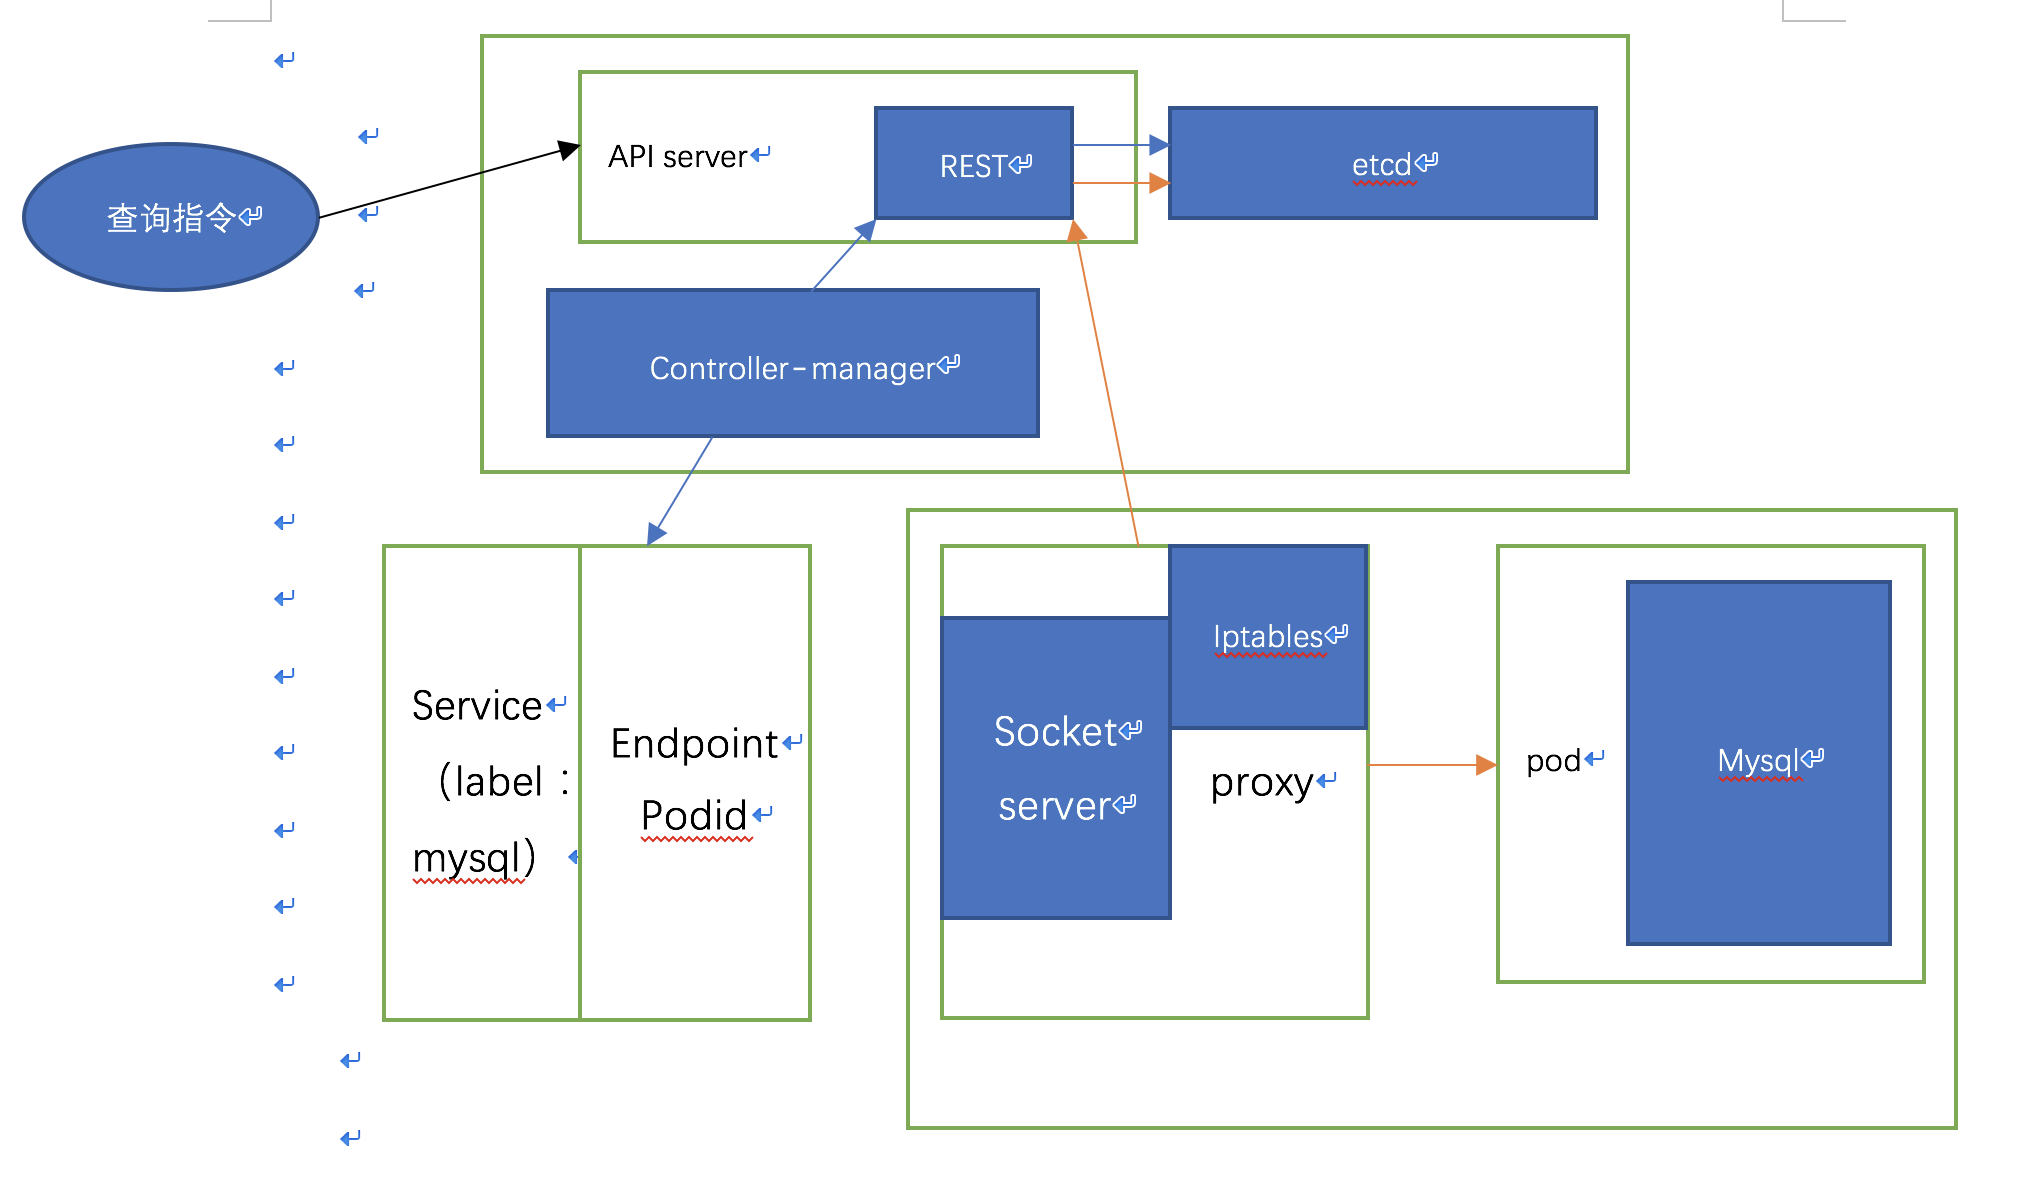
\includegraphics[scale=0.4]{visit_pod.png}
    \caption{访问pod}
    \label{fig:visit_pod}
\end{figure}
\begin{enumerate}
    \item controller-manager会监控API server的端口,然后管理service和endpoint的创建,其中endpoint主要是提供了server对应pod 的副本的访问地址
    \item proxy是service的主要实现者,他通过监听API server的端口,发现service,为service创建一个代理接口socket server用来接收来自server的访问请求,并创建Iptables,利用其规则使service的请求重定向到socket server。
    \item 在收到service请求之后,proxy将请求转发到后端的pod上,实现请求并实现负载均衡
\end{enumerate}

\section{kubernetes基本操作}

\subsection{NameSpace}
\begin{code-block}{bash}
# 查看所有namespace
kubectl get namespace
# 查看所有namespace,并包含lable信息
kubectl get namespace --show-labels
# 查看namespace的详细信息
kubectl describe namespace kube-system
# 从命令行新建namespace
kubectl create namespace zhangjl

# 从文件创建namespace
cat >zhangjl.yml<<EOF
apiVersion: v1
kind: Namespace
metadata:
  name: zhangjl
EOF
kubectl create -f zhangjl.yml

# 新建带有lable的namespace
cat >zhangjl.yml<<EOF
apiVersion: v1
kind: Namespace
metadata:
  name: zhangjl
  labels:
    namespace-name: zhangjl
    owner: zhangjl
EOF
kubectl create -f zhangjl.yml
\end{code-block}

\subsection{Contenxt}
\begin{code-block}{bash}
# 获取所有上下文环境
kubectl config get-contexts

# 查看context的具体信息
kubectl config view

# 查看当前使用的context
kubectl config current-context

# 新增context
kubectl config set-context zhangjl --namespace=zhangjl --cluster=kubernetes --user=admin

# 切换至新的context
kubectl config use-context zhangjl

\end{code-block}


\subsection{Pod}

\subsection{Replication}

\subsection{Deployment}